\documentclass[twocolumn,10pt]{article}
\usepackage[margin=2cm,headheight=21pt]{geometry}
\usepackage{amsmath,amssymb,amsthm,etoolbox,graphicx}
\usepackage{ragged2e,booktabs,float,hyperref}
\usepackage[ruled,vlined]{algorithm2e}
\usepackage{xcolor}
\usepackage[skins,theorems,breakable,listings]{tcolorbox}
\usepackage{titlesec,fancyhdr,caption,colortbl,tikz}
\pagestyle{fancy}
\fancyhead[L]{Report dependency check}
\newtcbtheorem{result}{Result}{colback=green!5,colframe=green!40!black}{res}
\begin{document}
\section{Tables and algorithms}
\begin{tabular}{lc}
\toprule
Method & Value \\
\midrule
Example & 1 \\
\bottomrule
\end{tabular}
\begin{algorithm}[t]
\KwIn{A finite sequence}
\KwOut{The sum}
\For{each element}{Add it to the accumulator\;}
\Return{the accumulator}\;
\end{algorithm}
\section{Report styling}
\begin{result}{A styled result}{example}
\RaggedRight For every real number $x$, $x^2 \geq 0$.
\end{result}
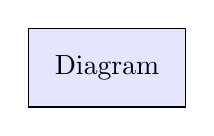
\begin{tikzpicture}
\draw[fill=blue!10] (0,0) rectangle (2,1);
\node at (1,0.5) {Diagram};
\end{tikzpicture}
\begin{tcblisting}{listing only,breakable}
result = sum(values)
\end{tcblisting}
\end{document}
